\section{Singular Value Decomposition}
The Singular Value Decomposition (SVD) is a matrix factorization with guaranteed existance.
It can be used to obtain low rank approximations of a matrix or pseudo inverses for ill posed linear system of equations.
It is also related to FT by providing a data specific set of orthogonal bases instead of a gerneric set of sines and cosines. For this paper the SVD will be used for generating low rank approximations of matrices.
\cite{brunton_kutz_2019b}
\subsection{Properties}
A matrix \(X \in \mathbb{C}^{n \times m}\) can be decomposed in the following way:
\begin{gather}
X = U \Sigma V^{*}
\end{gather}
Here \(U \in \mathbb{C}^{n \times n}\) and \(V \in \mathbb{C}^{m \times m}\) are unitary matrices and \(\Sigma \in \mathbb{R}^{n \times m}\) is a real valued oredered diagonal matrix.
The columns of \(U\) provides a set of orthonormal basis vectors for the column space of \(X\), \(V\) contains orthonormal basis vectors for the row space of \(X\). The matrix \(\Sigma\) asigns a magnitude ('importance') to the product of \(U\) and \(V^{*}\)  \cite{brunton_kutz_2019}.
Since \(U\) and \(V\) are unitary they have the following property:
\begin{gather}
U^{*}U = UU^{*} = I \\
V^{*}V = VV^{*} = I
\end{gather}
\cite{SZABO2015385}


In case \(n \geq m\) the so called economy SVD can be used to factorize the matrix \(X\):
\begin{gather}
X = \begin{bmatrix}
\hat{U} & \hat{U}^{\bot}
\end{bmatrix} 
\begin{bmatrix}
\hat{\Sigma} \\
0
\end{bmatrix}
V^{*} = \hat{U} \hat{\Sigma} V^{*}
\end{gather} 
The economy SVD omits rows only containing zeros in \(\Sigma\) and the according columns of \(U\).
Therefore the dimensionality of \(\hat{U}\) and \(\hat{\Sigma}\) is less or equal to the dimensionality of \(U\) and \(\Sigma\).
 \cite{brunton_kutz_2019b}

\subsection{Hirachy of correlations}
As alaready stated, the matrix \(\Sigma\) assigns a magnitude to \(UV^{*}\).
This magnitude can be seen as the square of the variance the bases in \(U\) and \(V\) capture.
Assume that \(X^{*}X\) and \(XX^{*}\) denote a correlation matrix.
\cite{brunton_kutz_2019}
A correlation matrix is a matrix that stores correlation coefficiants between multible measurements. 
If \(X\) has the following properties \(X^{*}X\) and \(XX^{*}\) are correlation matrices:
\paragraph{1.) The column vectors of \(X\) have to be zero mean:}
\begin{gather}
X = \begin{bmatrix}
x_1, \hdots, x_m
\end{bmatrix} \\
\frac{1}{n}\sum_{j = 1}^{n} x_{ij} = \mu_{i} = 0 \quad \forall 1 \leq i \leq m
\end{gather}
\paragraph{2.) The column vectors of \(X\) have to be normalized:}
\begin{gather}
(\sum_{j = 1}^{n} x_{ij}^{2})^{\frac{1}{2}} = \bar{x_i} = 1 \quad \forall 1 \leq i \leq m
\end{gather}
The correlation coefficiant between two column vectors of \(X\) is calculated as follows:
\begin{gather}
corr(x_i, x_{i'})\frac{(\sum_{j = 1}^{n} x_{ij} - \bar{x_i})(\sum_{j = 1}^{n} x_{i'j} - \bar{x_{i'}})}{(\sum_{j = 1}^{n} (x_{ij}- \bar{x_{i}})^{2})^{\frac{1}{2}}(\sum_{j = 1}^{n} (x_{i'j}-  \bar{x_{i'}})^{2})^{\frac{1}{2}}}
\end{gather}
\cite{Suga}


Since all coloumn vectors have zero mean and are normalized this becomes:
\begin{gather}
corr(x_i, x_{i'}) = cov(x_i, x_{i'})= x_i^{*}x_{i'}
\end{gather}
\cite{harv}


This resembles the entries of \(XX^{*}\) and \(X^{*}X\).
A vector \(e\) that maximizes the variance of the projecetions of \(x_i\) onto \(e\)  with the restriction \(||e|| = 1\) are the eigenvectors of the according correlation matrix.
The eigenvalue of \(e\) denoted as \(\lambda\) is eqiuvalent to the variance of \(x_i\) projected onto \(e\) \cite{Lavrenko}.

Since \(X\) can be deconstructed using the SVD, \(XX^{*}\) and \(X^{*}X\) are equal to:
\begin{gather}
XX^{*} = U\begin{bmatrix}
\hat{\Sigma} \\
0
\end{bmatrix}V^{*}V\begin{bmatrix}
\hat{\Sigma} & 0
\end{bmatrix}U^{*} = U \begin{bmatrix}
\hat{\Sigma}^{2} & 0 \\
0 & 0
\end{bmatrix} U^{*} \label{corr-1}\\
X^{*}X = V \begin{bmatrix}
\hat{\Sigma} & 0
\end{bmatrix} U^{*}U \begin{bmatrix}
\hat{\Sigma} \\
0
\end{bmatrix} V^{*} = V\hat{\Sigma}^{2}V^{*} \label{corr- 2}
\end{gather}
By multiplying \(U\) and \(V\) respectivley on the right side \ref{corr-1} and \ref{corr- 2} become:
\begin{gather}
XX^{*}U = U \begin{bmatrix}
\hat{\Sigma}^{2} & 0 \\
0 & 0
\end{bmatrix} \\
X^{*}XV = V\hat{\Sigma}^{2}
\end{gather}
This shows that \(V\) contains the eigenvectors of the row-wise correlation matrix and \(U\) contains the eigenvectors of the column-wise correlation matrix.
The matrix \(\Sigma\) contains the roots of the according eigenvalues and is thereby related to the variance.
By ordering \(U\), \(\Sigma\) and \(V\) by the entries of \(\Sigma\) in a descending order he first row of \(U\) and \(V\) contain the most important basis vectors. \cite{brunton_kutz_2019b}

\subsection{Low-rank approximation}
A usefull property of the SVD is that it can be used to find an hierachy of rank-\(r\) approximation for a given matrix \(X\).
An matrix \(\tilde{X}\) that approximates \(X\) is obtained by:
\begin{gather}
\tilde{X} = arg\,min ||X - \tilde{X}||_F = \tilde{U}\tilde{\Sigma}\tilde{V}^{*}	\\
s.t. rank(\tilde{X}) = r
\end{gather}	
Here  \(\tilde{U}\) and \(\tilde{V}\) denote matrices obtained takeing the first \(r\) columns of \(U\) and \(V\). The matrix \(\tilde{\Sigma}\) is a \(r \times r\) sub-block of \(\Sigma\).
This is alsow known as the Eckard-Young theorem.
The variance captured by \(\tilde{X}\) can be calculated in the following way:
\begin{gather}
cumvar_{r}(\Sigma) = \frac{\sum_{i = 1}^{r} \sigma_i}{trace(\Sigma)} \label{cum-var-r} \\
var(\Sigma) = \frac{diag(\Sigma)}{trace(\Sigma)} \label{var-sig}
\end{gather}
\cite{brunton_kutz_2019b}
\subsection{Example low-rank approximation}
As an example suppose there is a matrix \(X \in \mathbb{Z}^{4\times4}\):
\begin{gather}
X = \begin{bmatrix}
3 & 1 & 5 & 5 \\
4 & -4 & 5 & 0 \\
-4 & -2 & -4 & 3 \\
5 & 1 & 5 & -4
\end{bmatrix}
\end{gather}
By computing the SVD the matrices \(U\), \(\Sigma\) and \(V\) are obtained.
Now \(\Sigma\) can be used to calculate the cummulative variance for an rank-\(r\) approximation and the variance captured by each basis vector of \(U\) and \(V\).
\pgfplotsset{width=6cm,compat=1.9}
\begin{figure}[H]
\centering
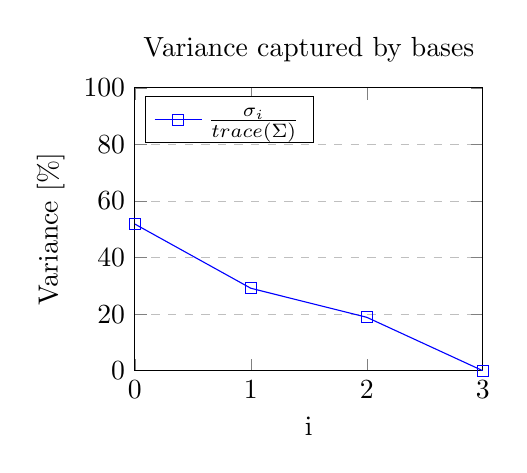
\begin{tikzpicture}
\begin{axis}[
    title={Variance captured by bases},
    xlabel={i},
    ylabel={Variance [\%]},
    xmin=0, xmax=3,
    ymin=0, ymax=100,
    xtick={0,1,2,3},
    ytick={0,20,40,60,80,100},
    legend pos=north west,
    ymajorgrids=true,
    grid style=dashed,
]

\addplot[
    color=blue,
    mark=square,
    ]
    coordinates {
    (0,51.87)(1,29.18)(2,18.91)(3,0.04)
    };
    \legend{\(\frac{\sigma_{i}}{trace(\Sigma)}\)}
    
\end{axis}
\end{tikzpicture}
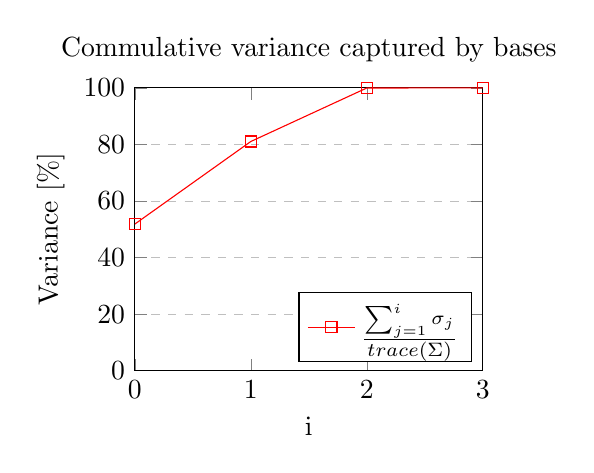
\begin{tikzpicture}
\begin{axis}[
    title={Commulative variance captured by bases},
    xlabel={i},
    ylabel={Variance [\%]},
    xmin=0, xmax=3,
    ymin=0, ymax=100,
    xtick={0,1,2,3},
    ytick={0,20,40,60,80,100},
    legend pos=south east,
    ymajorgrids=true,
    grid style=dashed,
]
\addplot[
    color=red,
    mark=square,
    ]
    coordinates {
    (0,51.87)(1,81.05)(2,99.96)(3,100)
    };
    \legend{\(\frac{\sum_{j=1}^{i}\sigma_{j}}{trace(\Sigma)}\)}

\end{axis}
\end{tikzpicture}
\label{var-plt}
\caption{Variance and commulative variance captured by each column vectors of \(U\) and \(V\)}
\end{figure}
On \ref{var-plt} the commulative variance and the variance of each basis vectors is plotted.
Here \(X\) can be apprixomated using the first three leading basis vectors.
This approximation captures already more than 99\% of the variance.
The resulting matrix \(\tilde{X}_3\) looks as follows:
\begin{gather}
\tilde{X}_3 = \begin{bmatrix}
4.73 & -0.76 & 5.62 \\
1.31 & -1.37 & 1.62 \\
-5.10 & -0.60 & 2.34
\end{bmatrix}
\end{gather}



